% Syntax-only wrapper; the deliverable transcription remains a fragment.
% This wrapper deliberately passes editorial bodies through unchanged. It
% checks their TeX content without imposing paragraph/strikeout restrictions.
% Required local TeX packages were unavailable at initial readiness check.
% Once available, run from work/validation:
% xelatex -interaction=nonstopmode -halt-on-error -file-line-error compile_wrapper.tex
\documentclass{article}
\usepackage{fontspec}
\usepackage{amsmath,amssymb}
\usepackage{tikz-cd}
\usetikzlibrary{shapes.geometric}
\usepackage[normalem]{ulem}

\newcommand{\cotefile}[1]{\par\bigskip\noindent\textbf{Cote #1}\par}
\newcommand{\scanpage}[1]{\par\medskip\noindent\textbf{Scan #1}\par}
\newcommand{\mspage}[1]{\par\noindent\textit{Manuscript page #1}\par}
\newcommand{\deleted}[1]{#1}
\newcommand{\inserted}[1]{#1}
\newcommand{\margin}[1]{#1}
\renewcommand{\uline}[1]{#1}
\renewcommand{\uuline}[1]{#1}
\newcommand{\diagram}[1]{#1}
\renewcommand{\figure}[1]{#1}
\newcommand{\unsure}[1]{#1}
\newcommand{\illegible}[1]{\ifmmode\text{[illegible: #1]}\else[illegible: #1]\fi}

\begin{document}
\cotefile{90}
\scanpage{2}
\deleted{\[f(gh)=\sum f_i(g)\varphi_i(h),\]}
\margin{\uline{$M$}}
\deleted{\illegible{1}}
\deleted{\unsure{fini et projectif|plat et projectif}}

\uline{Lemme 1} Soit $A$ un anneau de Dedekind, $M$ un $A$-module plat. \deleted{Conditions équivalentes} Pour $\forall$ sous-module $N$ de $M$, soit $\tilde N$ l'image inverse dans $M$ du sous-module de Torsion de $M/N$. Donc $\tilde N/N$ est un module de torsion.

\unsure{Cond.} équivalentes a) b) c) d)

a) $\forall\,N$ de type fini, $\tilde N/N$ est de longueur finie, i.e. $\tilde N$ est de t.f.

\deleted{\unsure{$A$ est un corps,}}
b) \inserted{Si $A$ n'est pas un corps,} Il n'existe pas de sous-module de $M$ isomorphe à :
\[
\inserted{A^{(p)}\unsure{=}\bigcup_n p^{-n}=\Gamma(S-\{p\},\underline O_S)\quad(S=\operatorname{Spec}A),}
\deleted{\unsure{K_p}}\quad p\text{ est un idéal maximal}
\]
de $A$ \deleted{$A$ est un corps.}

\deleted{\unsure{Pour tout}}
c) \inserted{Si $A$ n'est pas un corps,} Pour $\forall$ idéal maximal \deleted{\unsure{$p$}} de $A$, $M_p$ ne contient pas de \unsure{$A$-module} Isom. à $K$.

d) $M=\varinjlim M_i$, les $M_i\subset M$ de type fini et ``\unsure{saturés}'', i.e. \inserted{$M_i\longrightarrow M_j$ \unsure{ts que|tels que} $M_i$ fact direct dans $M_j$.}

Pour que ces conditions soient \deleted{\unsure{vraies}}, il suffit que l'on ait :

e) Les formes linéaires sur $M$ séparent, i.e.
\[
M\hookrightarrow A^I\qquad(I\text{ un ensemble})
\]
[condition vérifiée si $M$ contenu ds un libre, \deleted{\unsure{par}} i.e. $M$ projectif]

C'est aussi nécessaire si $M$ a un ens. dénombrable de générateurs.
\mspage{1}
\scanpage{3}
\mspage{2}
deux cas envisagés dans b), on voit que leur nombre est 1, donc que $B'$ est local. D'autre part, l'hypothèse $X\quad Y$ plat à fibres séparables est héritée par $\unsure{X'}=\operatorname{Spec}(B')\quad Y'=\operatorname{Spec}(A')$, et les fibres génériques sont isomorphes, ce qui nous permet de remplacer $f:X\quad Y$ par $f':X'\quad Y'$, donc de supposer $Y$ géométriquement unibranche. (Ceci montre d'ailleurs que 19.9.7 est essentiellement contenu dans son corollaire 18.9.11).

Compte tenu de 15.5.6.1. nous sommes ramenés à prouver alors que pour tout $x\quad X$ tel que $f(x)=y$ ne soit pas maximal, $\operatorname{Spec}(\underline{\mathrm O}_{X,x})$ n'est pas disconnecté par $x$. Changeant de notations, on est ramené à prouver que lorsque $\dim Y\quad1$, alors $X$ n'est pas disconnecté par son point fermé $x$. Notons que
\[
\operatorname{prof}B=\operatorname{prof}A+\operatorname{prof}B\otimes_A k
\]
et comme $\operatorname{prof}A\quad1$, puisque $A$ est intègre de dimension 1, on voit que $\operatorname{prof}(B)\quad2$ \uline{sauf} si $\operatorname{prof}B\otimes_A k=0$, ce qui équivaut à $\dim B\otimes_A k=0$ puisque par hypothèse $B\otimes_A k$ est séparable sur $k$, donc \deleted{\unsure{intè}} réduit. Or si $\operatorname{prof}B\quad2$, la conclusion voulue résulte du th. de Hartshorne. \deleted{\unsure{D'autre}}

D'ailleurs, si $A$ est normal, \deleted{\unsure{et de dimension}} et si $\dim A\quad2$, on a $\operatorname{prof}A\quad2$ d'où $\operatorname{prof}B\quad2$, d'où encore la conclusion voulue. Dans le cas où l'anneau $A$ envisagé dans 18.9.7. est universellement \deleted{\unsure{catégnaire|caténaire}, \unsure{(hypothèse}}\inserted{japonais} \inserted{on peut observer que} \deleted{\unsure{envisagée}} dans les réductions précédentes, on peut (sans invoquer 0 23.2.5\unsure{)} se ramener \deleted{\unsure{directe}} tout de suite au cas $A$ normal (en prenant pour $A'$ le normalisé de $A/\underline p$ dans une extension finie donnée de son corps des fractions), et par suite \deleted{on} l'argument qui précède montre qu'on est réduit au cas où $A$ est de plus de dimension 1, donc spectre d'un anneau de val discrète, et où $B\otimes_A k$ est de dimension 0, donc réduit à un corps, puisqu'il est réduit, ce qui implique aussitôt que $B$ est lui-même un anneau de valuation discrète, donc $X-x$ est réduit à un point et par suite connexe.
\scanpage{4}
\uline{Lemme 2} Soit \deleted{$\unsure{B}$} $A$ comme dessus, $G$ un $A$-groupe affine, d'algèbre $B$, satisfaisant les conditions ci-dessus. Alors pour \unsure{tt} sous-module de type fini $M$ de $B$, $\exists$ sous-module de type fini $N$ de $B$ tel que $N\supset M$ et tel que

a) $\tilde N=N$ i.e. $N$ saturé --- ce qui implique $N\otimes_A N\hookrightarrow B\otimes_A B$

b) $\Delta N\subset N\otimes N$

\uline{Dém.} Faisons opérer $G\times G$ \deleted{$\unsure{\longrightarrow}$} sur $B$ par
\[
(g,h)f(s)=f(g^{-1}sh).
\]
\deleted{Alors \unsure{le}} Un sous-module $N$ de $B$ est invariant par $G\times e$ (resp $e\times G$) \deleted{\unsure{ssi}} ssi on a
\[
\Delta N\subset N\otimes B\qquad\text{resp.}\quad\Delta N\subset B\otimes N.
\]
Notons que \deleted{grâce à la platitude de $B$, cette} chacune de ces conditions est stable par passage de $N$ à $\tilde N$. (faire l'argument).

Donc, la condition d'être invariant par $G\times G$, qui est la conjonction des deux, est aussi stable par passage de $N$ à $\tilde N$. Or, on sait que $M\subset N$ \inserted{de t.f.} stable par $G\times G$. Par hyp., $\tilde N$ est encore de t.f., \deleted{\unsure{or}} et est encore stable. \inserted{on peut supposer $N=\tilde N$}

Mais \unsure{cela impliq.}
\[
\Delta\tilde N\subset(\tilde N\otimes B)\cap(B\otimes N)=N\otimes N
\]
cqfd.
\mspage{3}
\scanpage{5}
\mspage{4}
EGA IV 18.9.\qquad (\uline{Rabiots})

L'assertion de connexité faite dans 18.9.1. se généralise de la façon suivante:

\uline{Théorème} 18.9.7. Soit $A\quad B$ un homomorphisme local d'anneaux locaux noethériens, et supposons a) \inserted{$f:$} $\operatorname{Spec}(B)=X\quad\operatorname{Spec}(A)=Y$ est plat à fibres séparables, et b) $A$ est géométriquement unibranche, ou $A$ est unibranche et $k(B)$ une extension primaire de $k(A)$. Alors la fibres générique de $X$ sur $Y$ est connexe, et pour toute partie fermée $S$ de $Y$ distincte de $Y$, \deleted{\unsure{et} \illegible{1}} et tout fermé $T$ de $X$ contenu dans $f^{-1}(S)$, $X-T$ est connexe.

Signalons tout \unsure{des|de} suite les corollaires suivants:

\uline{Corollaire} 18.9.8. Supposons qu'on ait a) ci-dessus, et b') $A$ est strictement local, ou $A$ est local hensélien et $k(B)$ est une extension primaire de $k(A)$. Alors \uline{toutes} les fibres de $X$ sur $Y$ sont \uline{géométriquement connexes}.

En effet, soit $A\quad A'$ un homomorphisme local, avec $A'$ fini sur $A$, et soit $B'=B\otimes_A A'$, alors on constate aussitôt que les hypothèses faites sont encore vérifiées pour $A'\quad B'$. Ceci nous ramène, comme d'habitude, au cas où $A$ est intègre, et à vérifier que dans ce cas, la fibre générique de $f:X\quad Y$ est connexe. Mais nous sommes alors sous les conditions du théorème qui précède.

\uline{Corollaire} 18.9.9. Soit $A$ un anneau local noethérien hensélien, \deleted{\unsure{int}} universellement caténaire (i.e. réf\quad à fibres formelles séparables). Alors les fibres formelles de $A$, i.e. les fibres de $\operatorname{Spec}(\hat{\hat A})\quad\operatorname{Spec}(A)$, sont \inserted{géom.} connexes.

C'est en effet un cas particulier de 18.9.8. (l'extension résiduelle $k(\hat A)$ sur $k(A)$ est ici triviale, à fortiori primaire).
\scanpage{6}
\uline{Corollaire} Si \inserted{de plus} $G$ est de t.f. sur $A$, alors $G$ admet une représentation linéaire fidèle.
\figure{\begin{tikzpicture}[x=1cm,y=1cm]\draw (0,0)--(-.03,.65);\end{tikzpicture}}

Il existe $N$ tel que a) $N$ engendre l'algèbre $B$, b) $\tilde N=N$, c) $\Delta N\subset N\otimes B$. \deleted{\unsure{le}} Alors \deleted{\unsure{le}} \unsure{tt} pt de $G$ à valeurs dans $A'/A$ qui opère \unsure{trivialt} sur $N'$, opère \unsure{trivialt} sur $B'$, \deleted{\unsure{et par suite}} donc est \deleted{\unsure{sur}} l'unité. Donc la repr. est fidèle.

\uline{Corollaire} Si $A$ est un corps $k$, alors, \unsure{tt} groupe affine \deleted{\unsure{de}} $G$ sur $k$ est lim. \deleted{\unsure{inductive}} projective d'un syst. projectif strict (\unsure{morph.} de transition des morphismes fid plats) de groupes affines \uline{de t.f.}.
\mspage{5}
\scanpage{7}
\mspage{6}
\mspage{-3-}
\uline{Corollaire} (18.9.5) .- \uline{Sous les hypothèses de} (18.9.4), \uline{le foncteur}
\[
(18.9.5.1)\qquad Z\rightsquigarrow Z\otimes_A A'
\]
\uline{de la catégorie des préschémas étales sur} $X$, \uline{dans celle des préschémas étales sur} $X'$, \uline{est pleinement fidèle}.

Soient $Z_1,Z_2$ deux préschémas étales sur $X$, et\deleted{\unsure{X}} posons $Z_{\unsure{1|i}}'=Z_{\unsure{1|i}}\otimes_A A'$ $(\unsure{1|i}=1,2)$ ; \deleted{\illegible{2}} il s'agit de prouver que tout $X'$-morphisme $Z_1'\to Z_2'$ provient, par changement de base, d'un \inserted{$X$-}morphisme unique $Z_1\to Z_2$. Supposons d'abord que \deleted{$Z_1$ et} $Z_2$ soi\deleted{en}t \uline{séparé\deleted{s}} sur $X$ ; alors, comme $\operatorname{Hom}_X(Z_1,Z_2)$ s'identifie à \deleted{\illegible{1}} $\Gamma(Z_1\times_X Z_2/Z_1)$, et que $Z_1\times_X Z_2$ est étale et séparé sur $Z_1$, $\operatorname{Hom}_X(Z_1,Z_2)$ s'identifie fonctoriellement, en vertu de (17.9.3), à l'ensemble des parties ouvertes et fermées $U$ de $Z_1\times_X Z_2$ telles que la restriction à $U$ de la projection $p:Z_1\times_X Z_2\to Z_1$ soit un morphisme surjectif et radiciel. L'assertion résulte donc dans le cas considéré de (18.9.4) et de ce que $Z_1'\times_{X'}Z_2'= {}=(Z_1\times_X Z_2)\otimes_A A'$.
\margin{\figure{
\begin{tikzpicture}[x=1cm,y=1cm]\draw (0,0)--(-.03,.3) (.02,.13)--(.48,.18) (.48,.06)--(.47,.33);\end{tikzpicture}}}

Passons au cas général ; il suffira de prouver que le graphe $\Gamma'$ d'un $X'$-morphisme $Z_1'\to Z_2'$, \inserted{qui est \uline{ouvert} (17.9.3) \inserted{dans $Z_1'\times_{X'}Z_2'$}} est de la forme $\Gamma\otimes_A A'$, où $\Gamma$ est \deleted{\illegible{1}} induit sur une partie \uline{ouverte} de $Z=Z_1\times_X Z_2$. En effet, la restriction à $\Gamma$ de la projection $p:Z\to Z_1$ est alors un \uline{isomorphisme}, car par changement de base \inserted{$A\to A'$} cette restriction devient l'isomorphisme restriction à $\Gamma'$ de la projection $p':Z'\to Z_1'$ (avec $Z'=Z\otimes_A A'$), et il suffit d'appliquer (2.7.1,(viii)) ; la conclusion résulte donc \inserted{alors} de la caractérisation des graphes de morphismes (\uline{I},5.3).
\margin{\figure{\begin{tikzpicture}[x=1cm,y=1cm]\draw (0,0) .. controls (.15,.18) and (.27,.2) .. (.4,.18) .. controls (.51,.16) and (.55,.25) .. (.52,.36);\end{tikzpicture}}}

Si $q:Z'\to Z$ est la projection canonique, pour prouver que $\Gamma'$ est de la forme \deleted{\illegible{1}} $q^{-1}(\Gamma)$, où $\Gamma$ est ouvert \inserted{dans $Z$}, il suffit, puisque $q$ est un morphisme \inserted{fidèlement} plat \inserted{et quasi-compact}, de prouver \deleted{\illegible{1}} qu'il existe un ensemble $U\subset Z$ tel que $\Gamma'=q^{-1}(\unsure{U})$ (2.3.12). Posons $Z''=Z'\times_Z Z'=Z\times_X X''$, où $X''=X'\times_X X'$, et soient $q_1:Z''\to Z'$, $q_2:Z''\to Z'$ les projections canoniques. Appli-
\scanpage{8}
\uline{Prop.} $A$ anneau, $G$ groupe affine sur $A$, d'algèbre $B$. On suppose que en tant que $A$-module, on a
\[
B=\varinjlim B_i,
\]
où $B_i\subset B$ sont tels que a) $B/B_i$ est plat$/A$, \deleted{b)} donc \deleted{$\unsure{\Delta}$} $B_i\otimes B_i\subset B\otimes B$, et b) $\Delta B_i\subset B_i\otimes B_i$.

\deleted{Soit} c) les $B_i$ sont projectifs de t.f.

\deleted{Alors} Pour $i$ fixe, utilisant a), on voit que pour \unsure{tt} $A$-module $E$, $B_i\otimes E\subset B\otimes E$.

Si $G$ opère sur $E$, disons que $E$ est $i$-admissible si $\delta:E-B\otimes E$ se factorise par $B_i\otimes E$, donc est défini par
\[
\delta_i:E-B_i\otimes E.
\]
Alors la catégorie des $A$-$G$-modules \inserted{de t.f.} est la limite inductive, pour $i$ variable, des sous-catégories $\unsure{\mathcal C_i(A,G)_f}$ des $A$-$G$-modules $i$-admissibles \inserted{de t.f.}. D'autre part, utilisant b) et c), et introduisant $\mathcal U_i=\check B_i$, on trouve que $\mathcal U_i$ est une algèbre ass. unitaire \deleted{\unsure{libre}}.

\deleted{\unsure{sur $A$} \illegible{2} \unsure{ainsi} \unsure{que} $\unsure{\varepsilon(B_i)=A}$, \unsure{la flèche} $\unsure{A\subset B}$.}

Alors, \deleted{la catégorie $\mathcal C_i$} $\mathcal U_i$
\mspage{7}
\scanpage{9}
\mspage{8}
\mspage{IV-965}
\uline{Corollaire} (18.9.4) .- \uline{Soit} $A$ \uline{un anneau local noethérien, hensélien et dont les fibres formelles sont géométriquement normales} \deleted{\illegible{1}} (par exemple un anneau local noethérien hensélien et \uline{excellent}), \uline{et posons} $A'=\hat A$. \uline{Soient} $X$ \uline{un} $A$-\uline{préschéma}, $X'=X\otimes_A A'$, $g:X'\to X$ \uline{la projection canonique. Alors l'application} $U\rightsquigarrow g^{-1}(U)$ \uline{est une bijection de l'ensemble des parties à la fois ouvertes et fermées de} $X$ \uline{sur l'ensemble des parties à la fois ouvertes et fermées de} $X'$.

Comme $g$ est un morphisme \deleted{\illegible{1}} fidèlement plat et quasi-compact, on sait (2.3.12) que la topologie de $X$ est \uline{quotient} de celle de $X'$ par la relation d'équivalence définie par $f$. Tout revient donc à voir \deleted{\unsure{que}} qu'une partie ouverte et fermée $U'$ de $X'$ est \uline{saturée} pour cette relation. Or, comme le morphisme $\operatorname{Spec}(A')\to\operatorname{Spec}(A)$ \deleted{\illegible{1}} a ses fibres géométriquement connexes (18.9.1), les fibres de $g$ sont \uline{connexes}, d'où aussitôt notre assertion.

En particulier, si $X$ est localement connexe (ce qui sera le cas si $X$ est localement noethérien), alors, pour toute \deleted{\unsure{partie}} composante connexe $U$ de $X$ (qui est ouverte et fermée dans $X$), $g^{-1}(U)$ est connexe (Bourbaki, \uline{Top.gén.}, chap.I, $3^e$ éd., \S\ 11, $n^\circ3$, \inserted{prop 7}). Si l'on désigne par $\pi_0(X)$ l'ensemble des composantes connexes de $X$, , l'application $\pi_0(X')\to\pi_0(X)$ déduite canoniquement de $g$ est donc \uline{bijective}.

\margin{``séparés'' inutile !}
\deleted{
\uline{Corollaire} (18.9.5) .- \uline{Sous les hypothèses de} (18.9.4), \uline{le foncteur}
\[
(18.9.5.1)\qquad Z\rightsquigarrow Z\otimes_A A'
\]
\uline{de la catégorie des} \deleted{$X$-}\inserted{pré}\uline{schémas étales} \inserted{\deleted{(resp. étales et finis)} (et séparés)} \uline{sur} $X$ \uline{dans celle des} \deleted{\illegible{1}}\inserted{pré}\uline{schémas étales} \inserted{\deleted{(resp. étales et finis)} (et séparés)} \uline{sur} $X'$, \uline{est pleinement fidèle}.

En effet, si $Z_1,Z_2$ soit deux $X$-schémas étales sur $X$, $\operatorname{Hom}_X(Z_1,Z_2)$ s'identifie à $\Gamma(Z_1\times_X Z_2/Z_1)$, et $Z_1\times_X Z_2$ est étale et séparé sur $Z_1$, donc finalement (17.9.3), $\operatorname{Hom}_X(Z_1,Z_2)$ s'identifie fonctoriellement à l'ensemble des parties ouvertes et fermées $U$ de $Z_1\times_X Z_2$ telles que la restriction de la projection $p:Z_1\times_X Z_2\to Z_1$ à $U$ soit un morphisme surjectif et radiciel. \unsure{Le|La} corollaire résulte donc aussitôt de (18.9.4) et du fait que, si $Z_{\unsure{1|i}}'=Z_{\unsure{1|i}}\otimes_A A'$ \deleted{\illegible{1}} $(\unsure{1|i}=1,2)$, on a $Z_1'\times_{X'}Z_2'=(Z_1\times_X Z_2)\otimes_A A'$.

\uline{Remarques} (18.9.6) .- (i) \deleted{Dans tous les cas connus} \inserted{il est possible que si le corps résiduel de $A$ est de car. nulle,} le foncteur (18.9.5.1) \deleted{est}\inserted{induit}
}
\margin{\unsure{le resp.} n'ajoute rien ; $X$-schéma risque d'induire en erreur---}
\scanpage{10}

forment un syst. projectif \inserted{strict} d'algèbres sur $A$.
$\mathcal C_i(G)_f$ est équivalente \unsure{canoniqut} à la catégorie des $\mathcal U_i$-modules \inserted{de t.f.}. Et les foncteurs \unsure{transition} entre les $\mathcal C_i(G)$ sont isomorphes aux \deleted{\unsure{aux}} foncteurs \uline{restriction des scalaires}.

\uline{Corollaire} Sous les conditions précédentes, tt module \inserted{de t.f.} $E$ d'une représentation de $G$ est quotient d'un module \inserted{\uline{projectif}} de t.f. où $G$ opère.
\margin{\figure{
\begin{tikzpicture}[x=1cm,y=1cm]\draw (0,0)--(-.04,1.7);\end{tikzpicture}}}

\uline{Prop.} Soit $G$ gr. affine plat sur $A$ anneau de Dedekind, d'algèbre $B$ satisfaisant aux conditions du lemme 1. (NB. si $G$ est de t.f. cela signifie que pour tte composante irréd. de $G$, \uline{toutes} ses fibres sont non vides).

Soit \deleted{$A'$ une $A$-algèbre} $S'$ un schéma sur $S$, tel que sur $S$, tt module quasi-coh de t.f. \deleted{admette \unsure{un}} \inserted{soit isomorphe} à un quotient d'un module loc. libre de t.f. \deleted{Alors} (p.ex. $S$ est \unsure{noeth.} \unsure{imm. quasi-proj.|immers. quasi-proj.}, ou $S$ noeth. régulier). Alors tt

\mspage{9}
\scanpage{11}
\mspage{10}
\mspage{IV-\unsure{964|764}}

\uline{Pour que} $A$ \uline{soit unibranche} (resp. \uline{géométriquement unibranche), il faut et il suffit que} $\operatorname{Spec}(A)$ \uline{soit irréductible}.

\uline{Proposition} (18.8.1\deleted{3}\inserted{5}).-- \uline{Soit} $A$ \uline{un anneau local noethérien. Si} $A$ \uline{est universellement caténaire, il en est de même de} ${}^{\mathrm{hs}}A$.

La démonstration est la même que celle de (18.7.5).

\uline{18.9. Fibres formelles des anneaux noethériens henséliens}.

\uline{Théorème} (18.9.1).-- \uline{Soit} $A$ \uline{un anneau local noethérien hensélien, dont les fibres formelles sont géométriquement normales. Alors les fibres formelles de} $A$ \uline{sont géométriquement intègres} (donc \uline{géométriquement connexes}).

Les deux assertions de l'énoncé sont en fait équivalentes, un préschéma \inserted{localement noethérien} connexe et normal étant intègre. Comme toute $A$-algèbre intègre finie est un anneau local hensélien (18.5.9 et 18.5.10), il résulte de (7.3.16.2) que l'on est ramené à prouver que si l'on suppose de plus $A$ \uline{intègre}, alors la fibre du morphisme $\operatorname{Spec}(\hat A)\to\operatorname{Spec}(A)$ au point générique de $\operatorname{Spec}(A)$ est \uline{intègre}, ce qui résulte du

\uline{Corollaire} (18.9.2).-- \uline{Soit} $A$ \uline{un anneau local noethérien hensélien intègre, dont les fibres formelles sont géométriquement normales. Alors} $\hat A$ \uline{est inté-}\deleted{\illegible{1}}\uline{gre}.

En effet, il résulte de (18.8.12) que $A$ est unibranche, donc \deleted{\illegible{1}} le théorème résulte de l'hypothèse faite sur les fibres formelles de $A$ et de (7.6.3).

\uline{Corollaire} (18.\deleted{\unsure{8}}\inserted{9}.3).-- \uline{Sous les hypothèses de} (18.9.2), \uline{le corps des fractions} $L$ \uline{de} $\hat A$ \uline{est une extension séparable du corps des fractions} $K$ \uline{de} $A$, \uline{et} $K$ \uline{est algébriquement fermé dans} $L$.

\deleted{\unsure{La première assertion}} \deleted{\illegible{4}} \inserted{Cela} résulte de ce que la fibre du morphisme $\operatorname{Spec}(\hat A)\to{}\to\operatorname{Spec}(A)$ au point générique de $\operatorname{Spec}(A)$ est géométriquement \deleted{\unsure{normal}}intègre et de (4.3.2) \inserted{et (4.3.5)}.

\scanpage{12}

$\unsure{G_S|G_{S'}}$-module \deleted{\unsure{est}} qu. coh de t.f. est quotient d'un idem, qui est de plus \uline{loc. libre}.

\mspage{11}
\scanpage{13}
\mspage{12}
\mspage{IV-\unsure{963}}

\uline{briques séparables de} $\kappa(\underline p)$ (ce qui entraîne que les fibres du morphisme canonique $\operatorname{Spec}({}^{\mathrm{hs}}A)\to\operatorname{Spec}(A)$ sont \uline{géométriquement régulières}).

\uline{Corollaire} (18.8.\deleted{9}\inserted{12}).-- \uline{Soit} $A$ \uline{un anneau local noethérien. Pour que} ${}^{\mathrm{hs}}A$ \uline{possède une des propriétés suivantes} :

a) \uline{être un anneau de Cohen-Macaulay} ;

b) \uline{vérifier la condition} $(S_n)$ ;

c) \uline{être régulier} ;

d) \uline{vérifier la condition} $(R_n)$ ;

\margin{\figure{
\begin{tikzpicture}[x=1cm,y=1cm]\draw (1,2.1) .. controls (.95,1.4) and (1.15,.8) .. (1.3,.6);\draw (0,1.45) .. controls (0,.35) and (.6,.5) .. (1.2,.6);\draw (0,0) .. controls (.3,.4) and (.7,.55) .. (1.2,.6);\draw[line width=.8pt] (1.5,.76)--(1.53,.49);\draw (1.78,.72) .. controls (1.74,.61) and (1.74,.58) .. (1.82,.55);\draw (2.08,1.12)--(2.1,.13);\fill (2.09,.57) circle (.025);\end{tikzpicture}}}

\uline{il faut et il suffit que} $A$ \uline{possède cette même propriété}.

\uline{Corollaire} (18.8.1\deleted{0}\inserted{3}).-- \uline{Soit} $A$ \uline{un anneau semi-local noethérien. Pour qu'un idéal premier} $\underline p$ \uline{de} ${}^{\mathrm{hs}}A$ \uline{appartienne à} $\operatorname{Ass}({}^{\mathrm{hs}}A)$, \uline{il faut et il suffit que} $\underline p\in A$ \uline{appartienne à} $\operatorname{Ass}(A)$.

Les démonstrations sont les mêmes que celles de (18.6.9), (18.6.10) et (18.6.11) respectivement.

\uline{Proposition} (18.8.1\deleted{1}\inserted{4}).-- \uline{Soit} $A$ \uline{un anneau local ; les propriétés suivantes sont équivalentes} :

a) $A$ \uline{est géométriquement unibranche} (resp. \uline{réduit et géométriquement unibranche}).

b) \uline{Pour toute} $A$-\uline{algèbre locale essentiellement étale} $A'$, $\operatorname{Spec}(A')$ \uline{est irréductible} (resp. \uline{intègre}).

c) $\operatorname{Spec}({}^{\mathrm{hs}}A)$ \uline{est irréductible} (resp. \uline{intègre}).

On se ramène comme dans (18.6.1\deleted{\unsure{1}}\inserted{2}) au cas où $A$ est réduit [\uline{en utilisant (18.8.7.1),}] et l'équivalence de b) et c) se prouve comme dans (18.6.1\deleted{\unsure{1}}\inserted{2}) ; il en est de même du fait que a) entraîne c), en tenant compte de (18.8.7.1) et de la définition d'un anneau local intègre géométriquement unibranche. Enfin pour démontrer que c) entraîne a), gardons les mêmes notations que dans (18.6.1\deleted{\unsure{1}}\inserted{2}) ; il s'agit encore de voir que ${}^{\mathrm{hs}}B$ est intègre. Mais, par (18.8.7), ${}^{\mathrm{hs}}B$ est un anneau local de l'anneau semi-local $B\otimes_A({}^{\mathrm{hs}}A)$, qui s'identifie encore par platitude à un sous-anneau du corps $L$, donc est intègre ; il en est par suite de même de ${}^{\mathrm{hs}}B$, ce qui achève la démonstration.
\margin{?}

\deleted{\unsure{Proposition}} \inserted{\uline{Corollaire}} (18.8.1\deleted{2}\inserted{5}).-- \uline{Soit} $A$ \uline{un anneau \inserted{local} hensélien} (resp. \uline{strictement local})

\scanpage{14}

\deleted{\uline{Proposition} Soit $A$ anneau de Dedekind, $G$ gr. \inserted{plat} affine \inserted{de t.f.} sur $A$, d'algèbre $B$ satisfaisant aux conditions du lemme 1. \deleted{Alors} Soit $N$ comme dans le lemme 2, et considérons \deleted{\unsure{la}} la représentation de $G$ dans $N$ induite par la repr. régulière gauche. Alors l'hom. $G\to\underline{\operatorname{Aut}}(N)$ est un morphisme fidèlement plat}

\figure{\begin{tikzpicture}[x=1cm,y=1cm]\draw (0,0)--(12,.75);\end{tikzpicture}}

\[
\left\{\begin{array}{ll}
\underline B=\varinjlim B_i &\\
1)\quad B/B_i\text{ plat} & \deleted{\text{donc}}\quad B_i\otimes B_i\subset B\otimes B\\
2)\quad \Delta B_i\subset B_i\otimes B_i &\\
3)\quad B_i\text{ loc. libre de t.f.} &
\end{array}\right.
\]
\deleted{\unsure{Suppos.} $X$ \uline{quasi-cpt} \uline{qu. sép.}}

Soit $E$ un $\underline O_X G$-module quasi-coh., \deleted{\illegible{1}}

Alors 1) Pour tt sous-module quasi-coh. $F$ il existe un plus petit \unsure{$A$-module|$\underline O_X$-module} quasi-coh. $F'$ de $F$ \deleted{tel que} stable par $G$, et sa formation commute à tt changement de base plat. Si $F$ est de t.f. $F'$ itou.

2) Si $X$ quasi-compact quasi-séparé, alors $E$ est $\varinjlim$ de sous-modules \inserted{qu. coh.} de t.f. qui sont stables par $G$.

\inserted{\deleted{\unsure{Pour $X$ quasi-cpt quasi-sép.}} \unsure{Si} $X$ quasi-cpt quasi-sép.}

3) Soit $F\to E$ un hom., avec $F$ quasi-coh. \inserted{de t.f.} dont l'image engendre $E$. Alors il existe

\mspage{13}
\scanpage{15}
\mspage{14}
\mspage{-4-}

quant (4.5.19.1), il suffit de montrer que $q_1^{-1}(\Gamma')=q_2^{-1}(\Gamma')$. Mais c'est une propriété \deleted{\unsure{purement} \illegible{1}} qui est vraie si \deleted{\unsure{elle}} et seulement si elle l'est après chaque changement de base $\operatorname{Spec}(\kappa(x))\to X$, où $x$ parcourt $X$. Autrement dit, il suffit de prouver le corollaire lorsque $X$ est le \uline{spectre d'un corps} ; mais comme tout $X$-préschéma étale est alors automatiquement \uline{séparé} sur $X$ (17.6.2,c')), on est ramené au cas envisagé au début de la démonstration.

\margin{\figure{\begin{tikzpicture}[x=1cm,y=1cm]\draw (.15,.35)--(.08,.27)--(0,.1)--(.24,0);\end{tikzpicture}}}

\scanpage{16}

un $G$-hom \deleted{$E$} $F'-E$ surjectif, avec $F'$ de la forme $F\otimes\check B_i$ --- donc $F'$ loc. libre (de t.f.) si $F$ l'est.

4) Supposons $X$ qu. cpt qu. sép. et que tt module qu. coh de t.f. sur $X$ soit quotient d'un loc. libre de t.f. (p.ex. $X$ a des \unsure{faisceaux} inv. \unsure{amples}, ou $X$ noeth. régulier). Alors tt $\underline O_X$-$G$-module sur $X$ est $\simeq$ quotient d'un loc. libre de t.f.

\mspage{15}
\scanpage{17}
\mspage{16}
\mspage{IV-962}

que de $k$ ; il est alors immédiat que $K\otimes_k\Omega$ est composé direct d'un nombre fini de corps, tous isomorphes à la clôture séparable $K\Omega$ de $K$. D'autre part, l'anneau ${}^{\mathrm{hs}}A$ étant hensélien, $C\otimes_A({}^{\mathrm{hs}}A)$ est composé direct des anneaux locaux $(C\otimes_A({}^{\mathrm{hs}}A))_{\underline{q_{\unsure{1|i}}}}$, où $\underline{q_{\unsure{1|i}}}$ $(1\leq\unsure{1|i}\leq s)$ parcourt les idéaux maximaux de \deleted{$\unsure{C'}$} $C\otimes_A({}^{\mathrm{hs}}A)$, et ces anneaux locaux sont henséliens (18.5.10) et ont $K\Omega$ pour corps résiduel, donc sont strictement locaux (18.8.1). Posons pour abréger $C'=C\otimes_A({}^{\mathrm{hs}}A)$ et $C_{\unsure{1|i}}'=C'_{\underline{q_{\unsure{1|i}}}}$, qui est donc un anneau quotient de $C'$ ; soient $f:C\to C'$, $g:{}^{\mathrm{hs}}A\to C'$, $\varphi_{\unsure{1|i}}:C'\to C_{\unsure{1|i}}'$ les applications canoniques.

\diagram{\begin{tikzcd}[column sep=small,row sep=large]
C \arrow[r,"f"'] \arrow[rrr,bend left=22,"v"] & C' \arrow[r] & C_i' \arrow[r,shift right=.65ex,"w"'] & {}^{\mathrm{hs}}C \arrow[l,shift right=.65ex,"w'"'] \\
A \arrow[u] \arrow[r,"\unsure{\prime}"] & {}^{\mathrm{hs}}A \arrow[u,no head] \arrow[urr,"u"'] & &
\end{tikzcd}}

Soit $v:$ \deleted{$\unsure{C\to C'}$} \inserted{$C\to{}^{\mathrm{hs}}C$} l'homomorphisme canonique ; il existe \deleted{\unsure{d'abord}} un homomorphisme local et un seul $u:{}^{\mathrm{hs}}A\to{}^{\mathrm{hs}}C$ qui, par passage aux quotients, donne l'injection canonique $\Omega\to K\Omega$ \deleted{\unsure{(18.8.5)}} et tel que le composé $A\to C\xrightarrow{v}{}^{\mathrm{hs}}C$ soit égal au composé $A\to{}^{\mathrm{hs}}A\xrightarrow{u}{}^{\mathrm{hs}}C$ (18.8.5) ; donc il existe un unique homomorphisme local $w_0:C'\to{}^{\mathrm{hs}}C$ tel que $w_0\circ g=u$, $w_0\circ f=v$, et puisque ${}^{\mathrm{hs}}C$ est un anneau local, cet homomorphisme se factorise en $C'\xrightarrow{\varphi_i}C_{\unsure{1|i}}'\xrightarrow{w}{}^{\mathrm{hs}}C$ pour un indice $\unsure{1|i}$ bien déterminé, $w$ étant un homomorphisme local. D'autre part, l'anneau $C_{\unsure{1|i}}'$ étant strictement local, il existe un homomorphisme local $w':{}^{\mathrm{hs}}C\to C_{\unsure{1|i}}'$ qui, par passage aux quotients, donne l'automorphisme identique de $K\Omega$ et qui est tel que $w'\circ v=\varphi_{\unsure{1|i}}\circ f$ \deleted{\unsure{,}} \inserted{(18.8.5)}. On déduit d'abord de là que $w\circ w'$ est un endomorphisme de ${}^{\mathrm{hs}}C$ qui, par passage aux quotients \deleted{\unsure{à}}, donne l'automorphisme identique de $K\Omega$, donc est l'identité (18.8.5). D'autre part, , on a $w'\circ w\circ\varphi_{\unsure{1|i}}\circ f=w'\circ v=\varphi_{\unsure{1|i}}\circ f$, et $w'\circ w\circ\varphi_{\unsure{1|i}}\circ g=w'\circ u=\varphi_{\unsure{1|i}}\circ g$ ; d'où $w'\circ w\circ\varphi_{\unsure{1|i}}=\varphi_{\unsure{1|i}}$, autrement dit $w'\circ w$ est l'automorphisme identique de $C_{\unsure{1|i}}'$. CQFD.

\uline{Remarque} (18.\unsure{8|9}.\deleted{7}\inserted{10}.1).-- La démonstration de (18.8.7) n'utilise le fait que $B$ est une $A$-algèbre finie, que pour établir que $K\otimes_k\Omega$ est composé direct d'un nombre fini de corps. Or, cette dernière propriété est encore vérifiée lorsque l'on suppose que $B$ est une $A$-algèbre \uline{entière semi-locale} dont les idéaux maximaux $\underline{n_j}$ ont des corps résiduels de degrés séparables $[\kappa(\underline{n_j}):k]_s$ \uline{finis}.
\margin{\figure{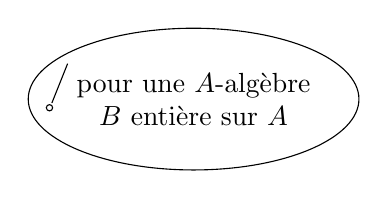
\begin{tikzpicture}\draw (0,0) ellipse (2.1 and .9);\node[align=center] at (0,0) {pour une $A$-algèbre\\$B$ \uline{entière} sur $A$};\draw (-1.8,-.05)--(-1.6,.45);\draw (-1.83,-.11) circle (.04);\end{tikzpicture}}}

\uline{Proposition} (18.8.\deleted{8}\inserted{11}).-- \uline{Soit} $A$ \uline{un anneau} \deleted{\unsure{noethérien}} \uline{semi-local}.

(i) \uline{Pour que} ${}^{\mathrm{hs}}A$ \uline{soit réduit} (resp. \uline{normal), il faut et il suffit que} $A$ \uline{le soit}.

(ii) \uline{Supposons} $A$ \uline{noethérien. Alors, pour tout idéal premier} $\underline p$ \uline{de} $A$, \uline{l'anneau} $({}^{\mathrm{hs}}A)_{\underline p}/\underline p\cdot({}^{\mathrm{hs}}A)_{\underline p}$ \uline{est composé direct d'un nombre fini d'extensions algé-}

\scanpage{18}

$G$ un groupe plat et affine sur $S$, d'algèbre $B$. On suppose
\[
B=\varinjlim B_i,\qquad B_i\subset B\quad\text{sous-Modules avec}
\]

1) $B/B_i$ plat (donc $B_i\otimes B_i\subset B\otimes B$)

2) $\Delta B_i\subset B_i\otimes B_i$ donc $\check B_i$ est un faisceau d'algèbres associatives à unité

3) $B_i$ \deleted{projectif} \inserted{loc libre} de t.f. avec les $\check B_i$ idem.

$X$ un préschéma sur $S$, \deleted{muni de $\uline{L}$ \uline{ample} rel/$S$} \inserted{où $G$ opère.}

\deleted{\unsure{Ainsi}} On suppose que sur $X$ existe un faisceau \inserted{inv} $\uline{L}$ ample rel/$S$, sur lequel $G$ opère de façon compatible avec son action sur $X$.

Soit $E$ un $\underline O_X$-$G$-Module quasi-coh. \deleted{\unsure{on suppose que}}

1) Pour tt sous-module qu. coh $F$ de $E$, il existe un plus petit sous-module qu. coh $F'$ de $E$ \deleted{qui} stable par $G$ \unsure{contt} $F$. Sa \deleted{\unsure{définition}} formation commute à tt changement de base plat en $S$.
\inserted{Si $F$ est de t.f., de $=$ $F'$.}

\deleted{2) Si $S$ qu. cpt qu. sép., alors $E$ est $\varinjlim$ de sous-modules quasi-coh. de t.f. qui sont stables par $G$.}
\margin{\deleted{t.f.}}

\mspage{17}
\scanpage{19}
\mspage{18}
\mspage{IV-953}

En effet, $Y$ étant compact \deleted{\unsure{et}} et noethérien, toute partie de $Y$ est compacte, donc fermée, ce qui implique que $Y$ est discret, donc fini puisqu'il est compact.

\uline{Corollaire} (18.6.10).-- \uline{Soit} $A$ \uline{un anneau local noethérien. Pour que} ${}^h A$ \uline{possède une des propriétés suivantes} :

a) \uline{être un anneau de Cohen-Macaulay} ;

b) \uline{vérifier la propriété} $(S_n)$ ;

c) \uline{être régulier} ;

d) \uline{vérifier la propriété} $(R_n)$ ;

\margin{\figure{
\begin{tikzpicture}[x=1cm,y=1cm]\draw (1,2) .. controls (.95,1.4) and (1.05,1.1) .. (1.35,1.05);\draw (0,1.6) .. controls (-.3,.7) and (.6,.7) .. (1.1,.85);\draw (0,0) .. controls (0,.5) and (.8,.6) .. (1.15,.7);\draw (1.25,.8) .. controls (1.05,.45) and (1.4,.4) .. (1.45,.65);\draw (1.4,.85)--(1.5,.65)--(1.6,.9)--(1.7,.8);\draw (1.5,1.05)--(1.65,1.1);\draw (1.85,1.1)--(1.9,.5);\draw (1.5,.8) ellipse (.6 and .45);\end{tikzpicture}}}

\uline{il faut et il suffit que} $A$ \uline{possède cette même propriété}.

Cela résulte aussitôt de ce que les fibres du morphisme $\operatorname{Spec}({}^h A)\to\operatorname{Spec}(A)$ sont géométriquement régulières (18.6.9) et de (6.4.1), (6.5.1) et (6.5.3).

\uline{Corollaire} (18.6.11).-- \uline{Soit} $A$ \uline{un anneau semi-local noethérien. Pour qu'un idéal premier} $\underline p$ \uline{de} ${}^h A$ \uline{appartienne à} $\operatorname{Ass}({}^h A)$, \uline{il faut et il suffit que} $\underline p\cap A$ \uline{appartienne à} $\operatorname{Ass}(A)$.

Compte tenu de la description des fibres du morphisme $\operatorname{Spec}({}^h A)\to\operatorname{Spec}(A)$, cela résulte aussitôt de (3.3.1).

\uline{Proposition} (18.6.1\deleted{\unsure{1}}\inserted{2}).-- \uline{Soi\deleted{\unsure{en}}t} $A$ \uline{un anneau local ; les propriétés suivantes sont équivalentes} :

a) $A$ \uline{est unibranche} (resp. \uline{réduit et unibranche}).
\margin{\figure{\begin{tikzpicture}[x=1cm,y=1cm]\draw (0,0) .. controls (0,.5) and (.25,.8) .. (.6,.85);\draw (.7,.9)--(.75,.82);\draw (.9,.9)--(.94,.86);\draw (1.1,1.05)--(1.18,.6);\end{tikzpicture}}}

b) \uline{Pour toute} $A$-\uline{algèbre locale strictement essentiellement étale} $A'$, \deleted{\unsure{Spec}} $\operatorname{Spec}(A')$ \uline{est irréductible} (resp. \uline{intègre}).

c) $\operatorname{Spec}({}^h A)$ \uline{est irréductible} (resp. \uline{intègre}).

Notons d'abord que ${}^h(A_{\mathrm{red}})=({}^h A)_{\mathrm{red}}$, car \deleted{\illegible{13}} ${}^h(A_{\mathrm{red}})=({}^h A)\otimes_A A_{\mathrm{red}}$ (18.6.8), et comme ${}^h(A_{\mathrm{red}})$ est réduit (18.6.9), il est égal à $({}^h A)_{\mathrm{red}}$. Ceci permet, dans la démonstration, de considérer seulement le cas où $A$ est \uline{réduit}, donc aussi $A'$ (17.5.7) et ${}^h A$ (18.6.9).

\deleted{\unsure{Il est clair que}} Avec les notations de (18.6.4), la condition b) signifie que tous les $A_\alpha$ sont intègres ; \deleted{comme les homomorphismes $\unsure{A_\alpha\to A_\beta|A_\alpha\to{}^h A}$ sont \unsure{injectifs}} on en conclut que ${}^h A=\varinjlim A_\alpha$ est intègre (5.13.3), donc b) entraîne c).

\scanpage{20}

\deleted{3) Si $\underline E$ est \deleted{de} de t.f. \inserted{et est quotient d'un Module loc libre (sans op.)} il existe un $\unsure{\underline O_X|\mathcal O_X}$-$G$-Module \deleted{\unsure{qui}} \uline{loc. libre de t.f.} $E$, et un épimorphisme de $\unsure{\underline O_X|\mathcal O_X}$-$G$-Modules $\underline F\longrightarrow E$.}

3) \deleted{Si $S$ est \unsure{et admet} un faisceau inv.} \inserted{qu. cpt \deleted{\unsure{quasi-sép.}} \inserted{qu. sép.} et si tt module quasi-coh.} de t.f. sur $S$ est $\simeq$ quotient d'un loc. libre de t.f., \deleted{ample,} alors $\underline E$ est $\simeq$ quotient d'un $\underline O_X$-$G$-Module loc. libre de type fini de la forme $f^*(H)(-n)$, \unsure{à}

\uline{Dém} Il suffit de prouver 1) et 3). Posons (où $f:X-S$)
\[
\underline{\Gamma}_{\deleted{*}}^\bullet(E)=\coprod_n f_*(E(n))
\]
Alors grâce au fait que $G$ est plat sur $S$ et $f$ qu. cpt et (qu) sép., on trouve que $\Gamma^\bullet(E)$ est un Module qu. coh sur $S$ sur lequel $G$ opère. Soit
\[
\underline{\Gamma}_{\deleted{*}}^\bullet(\unsure{\underline O_X|\mathcal O_X})=\deleted{\unsure{B^\bullet}}\mathcal A^\bullet
\]
c'est une Algèbre qu. coh sur laquelle $G$ opère. $E\unsure{\sim|\mapsto}\underline{\Gamma}^\bullet(E)$ est un foncteur en $E$, à valeurs dans les \deleted{\unsure{objets}} $\mathcal A^\bullet$-$G$-Modules qu. coh. Le foncteur est exact à gauche. On a un foncteur (\uline{exact})

\mspage{19}
\scanpage{21}
\mspage{20}
\mspage{IV-\unsure{952}}

\uline{neau} $({}^h A)_{\underline p}/\underline p\cdot({}^h A)_{\underline p}$ \uline{est} \deleted{\unsure{produit}} \uline{composé direct d'un nombre fini d'extensions algébriques séparables de} $\kappa(\underline p)$ (ce qui entraîne que les fibres du morphisme canonique $\operatorname{Spec}({}^h A)\to\operatorname{Spec}(A)$ sont \uline{géométriquement régulières}).

(i) Comme ${}^h A$ est un $A$-module fidèlement plat, il résulte de (2.1.13) que si ${}^h A$ est \deleted{\unsure{un}} réduit (resp. normal), il en est de même de $A$. Pour prouver la réciproque, on peut se borner au cas où l'anneau $A$ est local, de sorte \deleted{\unsure{à}} qu'avec les notations de (18.6.4), on a ${}^h A=\varinjlim A_\alpha$. Or, il résulte de la définition des $A_\alpha$ et de (17.5.7) que si $A$ est réduit (resp. intègre et intégralement clos), il en est de même des $A_\alpha$ ; \deleted{\unsure{en}} en outre, les \deleted{\illegible{2}} \deleted{\illegible{7}} morphismes \deleted{$\operatorname{Spec}(A_\beta)\to\operatorname{Spec}(A_\alpha)$} \inserted{$A_\alpha\to A_\beta$} pour $\alpha\leq\beta$ sont \deleted{surjectifs} \inserted{injectifs} en vertu de \deleted{(2.5.4,(ii))}. On conclut donc de (5.13.2) (resp (5.13.4)) que ${}^h A$ est réduit (resp. intègre et intégralement clos).
\margin{\unsure{précieux|curieux} \unsure{mélange !}}

(ii) \inserted{On peut se borner au cas où $A$ est local.} En vertu du fait que le foncteur $\varinjlim$ permute au produit tensoriel, la fibre du morphisme $\operatorname{Spec}({}^h A)\to\operatorname{Spec}(A)$ en un point $p$ est limite inductive des fibres des morphismes $\operatorname{Spec}(A_\alpha)\to\operatorname{Spec}(A)$ en ce point. . Comme ${}^h A$ est noethérien, on voit, compte tenu de (17.6.2), que l'on est ramené à prouver le lemme suivant :

\uline{Lemme} (18.6.9.1).-- \uline{Soient} \deleted{$\unsure{B}$} $(B_\alpha)$ \uline{un système inductif d'anneaux artiniens}, $B=\varinjlim B_\alpha$ \uline{sa limite inductive. Si} $B$ \uline{est noethérien, alors} $B$ \uline{est artinien} ; \deleted{\illegible{9}} \uline{si de plus, pour} $\alpha\leq\beta$, \uline{les homomorphismes} \inserted{$\varphi_{\beta\alpha}:$} $B_\alpha\to B_\beta$ \uline{sont injectifs, alors il existe} $\lambda$ \uline{tel que, pour} $\alpha\geq\lambda$ \uline{le nombre des composants locaux} \deleted{\unsure{de}} $B_\alpha^{(\unsure{1|i})}$ \uline{de} $B_\alpha$ \uline{soit constant}, \deleted{\unsure{de sorte}} \uline{que} $\varphi_{\beta\alpha}(B_\alpha^{(\unsure{1|i})})\subset B_\beta^{(\unsure{1|i})}$ \uline{pour tout} $\unsure{1|i}$ \uline{et que les} $B^{(\unsure{1|i})}=\varinjlim B_\alpha^{(\unsure{1|i})}$ \uline{soient les composants locaux de} $B$.

Soient en effet $Y_\alpha=\operatorname{Spec}(B_\alpha)$, $Y=\operatorname{Spec}(B)$, qui, en tant qu'espace topologique, est égal à $\varprojlim Y_\alpha$ (8.2.10). Les espaces $Y$ étant \deleted{\unsure{compacts}} \inserted{finis et} discrets, la seconde assertion du lemme résultera de la première et du fait que si les $\varphi_{\beta\alpha}$ sont injectifs, les morphismes canoniques $Y_\beta\to Y_\alpha$ sont surjectifs. On est ainsi ramené à prouver le lemme purement topologique suivant :
\margin{\unsure{peu clair}}
\margin{\figure{
\begin{tikzpicture}[x=1cm,y=1cm]\draw (0,1.6)--(-.02,.1)--(.1,0)--(.24,.02);\end{tikzpicture}}}

\uline{Lemme} (18.6.9.2).-- \uline{Soit} $(Y_\alpha)$ \uline{un système projectif d'espaces topologiques finis et discrets. Si} $Y=\varprojlim Y_\alpha$ \uline{est noethérien}, $Y$ \uline{est fini et discret}.

\scanpage{22}

$\unsure{M_\bullet}\sim\unsure{\widetilde M_\bullet}$ en sens inverse \inserted{(ils sont adjoints...)} et le composé \deleted{est} $E\sim\widetilde{\underline{\Gamma}(E)}$ est isom. à l'identité, ce qui montre que $\underline{\Gamma}^\bullet$ est \uline{pleinement fidèle}.

$F$ correspond à un sous-\deleted{$\unsure{\mathcal O}$} $\mathcal A^\bullet$-module $\Gamma^\bullet(F)$ de $\Gamma^\bullet(E)$, pas à priori stable par action de $G$. Si \deleted{$F'\supset F$ est} \inserted{$F'$, tel que} $F\subset F'\subset E$, \deleted{$F'\supset F$}, est stable par $G$, alors $\Gamma^\bullet(F')$ \deleted{$\Gamma^\bullet_{\deleted{*}}(\unsure{E'|F'})\subset\Gamma^\bullet(E)$}, satisfait
\[
\underline{\Gamma}^\bullet(F)\subset\underline{\Gamma}^\bullet(F')\subset\underline{\Gamma}^\bullet(E)\quad\text{est est stable par }G.
\]

On sait qu'il y a un plus petit sous-\inserted{$\unsure{\underline O_S|\mathcal O_S}$}-Module $N$ de $\Gamma^\bullet(E)$, \unsure{contt} $\underline{\Gamma}^\bullet(F)$, et stable par $G$. On voit tout de suite que $N$ est un sous-module gradué [\unsure{par ex.} $N\cap\Gamma^i(E)$ contient $\underline{\Gamma}^i(F)$, et est stable par $G$, donc contt le plus petit sous-module $M^i$ de $\underline{\Gamma}^i(E)$ contt $\underline{\Gamma}^i(F)$ et stable par $G$, donc $N$ contient $\sum M^i$, d'où par minimalité lui est égal]. De $=$, par fonctorialité de la construction de $N$, on voit que $N$ est un sous-$\mathcal A$-module. Considérons alors

\mspage{21}
\scanpage{23}
\mspage{22}
\mspage{IV-951}

et il est clair par (18.\unsure{6}.6,(v)) que si $A$ est noethérien \deleted{\unsure{,}}, il en est de même de ${}^h A$.

\deleted{Enfin, ${}^h A$ possède aussi la propriété universelle (18.6.6,(ii)) en convenant d'appeler ``homomorphisme \inserted{semi-}local'' de $A$ dans un anneau \inserted{semi-}local $B$ tout homomorphisme $\varphi$ tel que $\varphi(\underline r)$ soit contenu dans l'idéal maximal \inserted{$\underline n$} de $B$. En effet, il est clair que pour un tel homomorphisme, $\varphi^{-1}(\underline n)$ doit contenir l'un des $\underline m_{\unsure{1|i}}$ puisqu'il contient leur intersection, donc $\varphi^{-1}(\underline n)$ est égal à l'un des $\underline m_{\unsure{1|i}}$, et $\varphi$ se factorise \deleted{\unsure{donc}} en $A\to A_{\underline m_{\unsure{1|i}}}\to B$; d'où l'on conclut \deleted{\illegible{1}} que $\operatorname{Hom.loc}(A,B)\unsure{-|=}\prod_i\operatorname{Hom.loc}(A_{\underline m_{\unsure{1|i}}},B)$, et le fait que (18.6.6,(ii)) est encore valable lorsque $A$ est semi-local en découle aussitôt.}

\margin{\unsure{vider|virer}, (la forme hybride ici ne mérite pas le nom de ``\unsure{prop.} universelle'') ou bien \unsure{arranger} avec des ``hom $\frac12$ locaux'' dans des \unsure{anneaux semi-locaux}}

\uline{Proposition} (18.6.8). -- \uline{Soient $A$ un anneau semi-local, $B$ une $A$-algèbre semi-locale et entière sur $A$. Alors $B\otimes_A({}^h A)$ est une $B$-algèbre semi-locale isomorphe à ${}^h B$.}

\deleted{\illegible{13}} Comme $B\otimes_A({}^h A)$ est entier au-dessus de ${}^h A$, chacun de ses idéaux maximaux est au-dessus d'un des idéaux maximaux de ${}^h A$, donc au-dessus d'un idéal maximal de $A$, et comme $B$ est entière sur $A$, les idéaux premiers de $B$ au-dessus d'un idéal maximal de $A$ sont des idéaux maximaux de $B$, si bien que finalement un idéal maximal de $B\otimes_A({}^h A)$ a pour projections dans $\operatorname{Spec}({}^h A)$ et $\operatorname{Spec}(B)$ des idéaux maximaux; compte tenu de (18.6.6,(iii)) et de (\uline{I},3.4.9), on conclut que l'anneau $B\otimes_A({}^h A)$ est semi-local. En outre, pour tout anneau local hensélien \inserted{$C$}, $\operatorname{Hom.loc}(B\otimes_A({}^h A),C)$ est en correspondance biunivoque avec l'ensemble des couples $(\varphi,\psi)$ d'homomorphismes locaux $\varphi:B\to C$, $\psi:{}^h A\to C$ tels que les composés $A\to B\xrightarrow{\varphi}C$, $A\to{}^h A\xrightarrow{\psi}C$ soient égaux. Mais \deleted{\illegible{4}} en vertu de la correspondance biunivoque entre $\operatorname{Hom.loc}(A,C)$ et $\operatorname{Hom.loc}({}^h A,C)$, on voit que pour tout $\varphi\in\operatorname{Hom.loc}(B,C)$ il existe un $\psi$ et un seul ayant \deleted{les}\inserted{la} propriété\deleted{s} précédente\deleted{s}, donc l'application $\operatorname{Hom}(B\otimes_A({}^h A),C)\to\operatorname{Hom}(B,C)$ est bijective, ce qui prouve la proposition en vertu de l'unicité de la solution
\figure{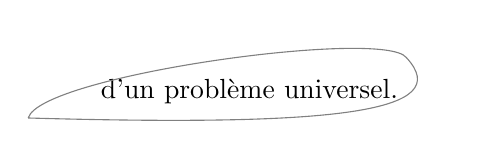
\begin{tikzpicture}[x=1cm,y=1cm]\node[anchor=west] at (0,0) {d'un problème universel.};\draw[gray] (-.8,-.34) .. controls (-.65,.2) and (3.7,.8) .. (4.0,.43) .. controls (4.65,-.27) and (3.1,-.45) .. (-.8,-.34);\end{tikzpicture}}

\margin{\uline{\unsure{Coroll.|cercle}}}

\uline{Théorème} (18.6.9). -- \uline{Soit $A$ un anneau semi-local.}

(i) \uline{Pour que ${}^h A$ soit réduit (resp. normal), il faut et il suffit que $A$ le soit.}

(ii) \uline{Supposons $A$ noethérien. Alors, pour tout idéal premier $\underline p$ de $A$, l'an-}
\scanpage{24}
\mspage{23}

$\widetilde N$, c'est un $\underline{O}_X$-$G$-module \deleted{\unsure{qui est contenu}} $\subset\inserted{\underline{\Gamma}^{\bullet}(F')=}\unsure{F'}$, et \deleted{contient} $\widetilde{\underline{\Gamma}^{\bullet}(F)}=F$. C'est donc le \deleted{\unsure{$F'$} cherché} faisceau cherché. Par construction, sa formation commute à \unsure{tt} changement plat $S'\to S$ de la base. Enfin, si $F$ est de type fini, \deleted{\unsure{alors $\exists$}} prouvons que son enveloppe $F'$ l'est. On peut supposer $S$ affine. Alors $\exists n$ tel que $F(n)$ \deleted{\unsure{pour $n$ assez gd}} engendré par ses sections, \deleted{soient alors}\inserted{donc par des} sections $\varphi_i$ \deleted{$\unsure{\in}$} $(1\leq i\leq N)$ $\in\Gamma(S,\underline{\Gamma}^n(F))$.

Considérons alors le sous-module \deleted{$\underline N^n$ de $\underline{\Gamma}^{\bullet}(E)$, engendré par les $\varphi_i$. Alors $\widetilde{\underline N}\subset F$ est en fait égal à $F$, comme on \unsure{const.} tt de suite. On peut donc répéter la construction \unsure{précédente}, en} $G$-invariant de $\underline{\Gamma}^{\unsure{n}}(F)$ engendré par les $\varphi_i$, soit $N^n$, et le sous Module de $\unsure{\underline E|E}$ qu'il définit. \uline{On vérifie} encore que c'est \uline{$F'$}, ce qui prouve que $F'$ est de type fini.....

\margin{Rédiger mieux \unsure{au début} de la démonstration, pour \unsure{pouvoir} \figure{\begin{tikzpicture}\draw[->] (0,0)--(.4,.45);\end{tikzpicture}} \unsure{y référer|la fois prochaine} \unsure{ici}.....}
\scanpage{25}
\mspage{24}
\mspage{IV-950}

$f_0^{(\lambda)}:S_0^{(\lambda)}\to S_0'{}^{(\lambda)}$ tels que $S'=S'{}^{(\lambda)}\times_{S^{(\lambda)}}S$, $\unsure{g|f}=\unsure{g|f}^{(\lambda)}\times1$ et $f_0=f_0^{(\lambda)}\times1$. \deleted{\illegible{1}} Soient $s$ le point fermé de $S$, $x=f_0(s)\unsure{_s}$, $x_\lambda$ la projection de $x$ dans $S'{}^{(\lambda)}$; comme $x_\lambda$ est au-dessus du point fermé de $S^{(\lambda)}$, l'anneau local \inserted{$\mathcal O_\lambda$} de $S'{}^{(\lambda)}$ au point $x_\lambda$ est une $A_\lambda$-algèbre essentiellement étale; en outre, comme $f_0^{(\lambda)}(s_\lambda)=$ $=x_\lambda$, on a $\kappa(x_\lambda)=\kappa(s_\lambda)$, autrement dit, $\mathcal O_\lambda$ est une $A_\lambda$-algèbre locale strictement essentiellement étale, et par suite (18.6.1) est $A_\lambda$-isomorphe à une $A$-algèbre $A_\mu$ avec $\mu\geq\lambda$. Il y a \deleted{\illegible{2}}\inserted{donc} un $A_\lambda$-homomorphisme \deleted{$\unsure{A_\mu\to A}$}\inserted{$\mathcal O_\lambda\to\unsure{A_\lambda|A}$}, c'est-à-dire un $S^{(\lambda)}$-morphisme $h:S\to S'{}^{(\lambda)}$ tel que $h(s)=x_\lambda$, et par suite il existe bien une $S$-section $f$ de $S'$ telle que $f(s)=x$, ce qui achève de prouver (i);

Pour prouver (ii), il suffit de noter que l'on a $\operatorname{Hom.loc}({}^h A,B)\deleted{\unsure{=}}$ $\deleted{=}\inserted{\simeq}\varprojlim\operatorname{Hom.loc}(A_\lambda,B)$ et que par (18.6.2) les homomorphismes canoniques $\operatorname{Hom.loc}(A_\lambda,B)\leftarrow\operatorname{Hom.loc}(A,B)$ sont bijectifs.

\deleted{\unsure{Enfin}} Pour démontrer \deleted{\unsure{le}} (iv), \deleted{\unsure{remarquons}} notons que pour tout $\lambda$ et tout entier $n>0$, $\underline m_\lambda^n=\underline m^n A_\lambda$, et $(\underline m.{}^h A)^n=\underline m^n.{}^h A=\varinjlim\underline m_\lambda^n$. On en conclut, par l'exactitude du foncteur $\varinjlim$ dans la catégorie des $A$-modules, que ${}^h A/(\underline m.{}^h A)^n=$ $=\varinjlim(A_\lambda/\underline m_\lambda^n)$, et par suite, il suffit de montrer que, pour tout entier $n$, et tout indice $\lambda$, l'homomorphisme $A/\underline m^n\to A_\lambda/\underline m_\lambda^n$ est bijectif. Or, \deleted{\unsure{pour}} cela est vrai par hypothèse pour $n=1$; d'autre part, puisque $A_\lambda$ est un $A$-module plat, on a
\[
\underline m_\lambda^n/\underline m_\lambda^{n+1}=(\underline m^n/\underline m^{n+1})\otimes_A A_\lambda=(\underline m^n/\underline m^{n+1})\otimes_{A/\underline m}(A_\lambda/\underline m A_\lambda)
\]
et comme $A/\underline m\to A_\lambda/\underline m A_\lambda=A_\lambda/\underline m_\lambda$ est bijectif, l'homomorphisme $\underline m^n/\underline m^{n+1}\to\underline m_\lambda^n/\underline m_\lambda^{n+1}$ est lui aussi bijectif; la conclusion résulte donc de Bourbaki, \uline{Alg.comm.}, chap.III,§ 2,n°8,\inserted{cor.3 du th.1}.

Enfin, si $A$ est hensélien \deleted{[et si $A'=B_{\underline n}$ est une $A$-algèbre locale strictement essentiellement étale, où $B$ est une $A$-algèbre étale, il résulte de \deleted{\unsure{la}} (18.6.2) qu'il existe une \deleted{\unsure{unique}} \uline{$\operatorname{Spec}(A)$-section de} $\operatorname{Spec}(B)$ prenant la valeur $\underline n$ au point fermé de $\operatorname{Spec}(A)$]}, on conclut \deleted{alors de}\inserted{de la remarque qui suit} (\deleted{17.4.1}\inserted{18.6.2}) que \deleted{\unsure{nécessairement}} \deleted{l'}\inserted{les}homomorphisme\inserted{s} \deleted{\unsure{canonique}} $A\to A\deleted{'}\inserted{_\lambda}$ \deleted{est}\inserted{sont} bijectif, ce qui prouve (vi) par définition de ${}^h A$.

(18.6.7) Soient maintenant $A$ un anneau \uline{semi-local}, $\underline m_{\unsure{1|i}}$ $(1\leq\unsure{1|i}\leq r)$ ses idéaux maximaux. On appelle \uline{hensélisé} de $A$ et l'on note encore ${}^h A$ l'anneau \uline{produit} $\prod_i{}^h(A_{\underline m_{\unsure{1|i}}})$ des hensélisés des anneaux locaux $A_{\underline m_{\unsure{1|i}}}$. C'est \inserted{un $A$-module fidèlement plat et} une $A$-algèbre semi-locale, dont les idéaux maximaux sont les $\underline m_{\unsure{1|i}}.{}^h A$ en vertu de (18.6.6,(iii)); en outre, si $\underline r=\bigcap_i\underline m_{\unsure{1|i}}$ est le radical de $A$, il résulte de ce qui précède que $\underline r.{}^h A$ est le radical de ${}^h A$ et que l'application $A/\underline r\to{}^h A/\underline r.{}^h A$ est bijective. Comme le séparé complété $\widehat A$ de $A$ pour la topologie $\underline r$-préadique est le produit des séparés complétés $\widehat{A_{\underline m_{\unsure{1|i}}}}$ (Bourbaki,\uline{Alg.comm.},chap.III,§ 2,n°13\inserted{prop.18}) l'homomorphisme canonique $\widehat A\to({}^h A)^\wedge$ est bijectif par (18.6.6,(iv)).
\cotefile{91}
\scanpage{2}

Représentabilité des

Foncteurs \uuline{Hom}, $\prod_{T/S}X/\unsure{T}$

de Greenberg etc.

\mspage{1}
\scanpage{3}

Représentabilité relative.

de $\prod_{X/S}P/X$

(sans hyp. \unsure{projectives})

\figure{
\begin{tikzpicture}\draw (0,0)--(1.6,0.04);\end{tikzpicture}}

``Flattening functor''

\figure{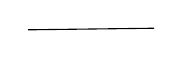
\begin{tikzpicture}\draw (0,0)--(1.6,0.02);\end{tikzpicture}}

Passage au quotient

\figure{
\begin{tikzpicture}\draw (0,0)..controls (.6,.07) and (1,.06)..(1.6,0);\end{tikzpicture}}

\[
\underline{\operatorname{Hom}}_S(X,Y)
\]
\[
\underline{\operatorname{Aut}}_S(X)
\]

\mspage{2}
\scanpage{5}
\mspage{4}

\uline{Th} $f:X\to S$ morphisme \inserted{\uline{plat}} de type fini, avec $S$ loc noeth, $Y$ \deleted{un sous-\unsure{préschém.} fermé de $X$}\inserted{$\to X$ un \unsure{mor.} de type fini}.

Pour que $\prod_{X/S}Y/X$ soit représentable, il f. et s. qu'il commute aux limites projectives adiques d'anneaux artiniens\inserted{, Si $Y\to X$ \unsure{une imm.} (\uuline{imm.f.})}, et alors il est représentable par un sous-préschém. (\uuline{fermé}) de $S$.

\margin{il suffit que $Y\to X$ soit un \uuline{\unsure{monomorphisme}}}

\figure{\begin{tikzpicture}\draw (0,0)--(10,0);\end{tikzpicture}}

\deleted{\unsure{fpqc}}

\uline{Dém.} Vérifions les conditions générales du th. de représentabilité pour morphismes non ramifiés séparés

1°) $F$ faisceau pour fpqc: \deleted{\unsure{EGA IV 2}} clair EGA IV 2

2°) $F$ commute aux $\varinjlim$ d'anneaux: clair EGA IV 8

\margin{$\times$ \unsure{N.B.}}

3°) C'est la condition de commutation aux $\varprojlim$ adiques d'artiniens.

4°), 5°), 6°) Dans le cas d'un monomorphisme $F\to S$ se réduit à ceci

\margin{\figure{
\begin{tikzpicture}\draw (0,0)--(.05,1.3);\end{tikzpicture}}}

si $A\to A'$ est un hom injectif d'artiniens \inserted{($A'/A$ fini)}

alors $F(A)\to F(A')$ est bijectif, ou même $F(A')\ne\varnothing\Rightarrow F(A)\ne\varnothing$. Il faut prouver que si $X_{A'}=Y_{A'}$, on a $X_A=Y_A$. C'est clair, car $X_A$ \deleted{\unsure{étant}} plat sur $A$, $\unsure{\underline O_{X_A}|\mathcal O_{X_A}}\deleted{\unsure{\otimes_A A}}\to\unsure{\underline O_{X_A}|\mathcal O_{X_A}}\otimes_A A'$ est injectif.

\margin{$\times$ \uline{plat}}

7°) Si $T$ sur $S$ est \deleted{\unsure{loc.}} loc. noeth., muni d'un idéal de carré nul $J$, $T_0=V(J)$, $U$ ouvert de $T$ tel que $T$ en soit l'adhérence schématique, \uline{alors} pour \deleted{$\unsure{F\subset F}$}
\diagram{\begin{tikzcd}
F(T) \arrow[r,dash] \arrow[d] & F(T_0) \arrow[d] \\
F(U) \arrow[r] & F(U_0)
\end{tikzcd}}
est cartésien.

\margin{$\times$ \uline{plat} \deleted{\uline{\unsure{Difficulté|fidèle}}}}
\scanpage{6}
\mspage{5}

\deleted{\uline{Théorème} $f:X\to S$ \inserted{plat} de présentation finie, $Y$ un sous-\unsure{préschéma} fermé de $X$ de présentation finie. Pour}
\scanpage{7}
\mspage{6}

\deleted{En d'autres termes}, si $F(T_0)\ne\varnothing$, $F(U)\ne\varnothing$, alors \deleted{$\unsure{\times}$} $F(T)\ne\varnothing$. \inserted{En fait, \inserted{lorsque $Y$ est \unsure{déjà} fermé dans $X$} il suffit ici $F(U)\ne\varnothing$ pour $F(T)\ne\varnothing$.} \deleted{\unsure{Donc} $X_{T_0}=Y_{T_0}$ et}\inserted{En d'autres termes si} $X_U=Y_U$, alors $X=Y$. En effet, comme $\unsure{T|S}$ est l'adhérence schématique de $U$ et $X_T$ plat sur $T$, $X_{\unsure{T}}$ est l'adhérence schématique de $X_U$, donc \deleted{\unsure{magique}} $Y_T=X_T$ puisque $Y_T$ sous-préschéma fermé de $X_T$ \unsure{renferme} $X_U$.

8°) Si $T$ sur $S$ irréductible muni \deleted{de} $J$ de carré nul, $T_0=V(J)$, si $F(T_0)\ne\varnothing$, \deleted{alors $\exists$ ouvert dense \unsure{de} $F(\unsure{\underline O_{T,\eta}|\mathcal O_{T,\eta}})\ne\varnothing$} alors $\exists$ ouvert dense $U$ de $T$ \deleted{sur lequel $F$} tel que $F_U$ repr.

En effet, il suffit que $\unsure{X}_U$ soit ``ess. libre'' sur $U$, et on sait qu'on peut trouver $U$ de cette façon EGA IV 11

\margin{$\times$ \unsure{par t.f.}}

De plus, on a vérifié 7° sous la forme plus forte \unsure{impliquant} que le foncteur est \uuline{propre}.

\deleted{\uline{Corollaire} \unsure{So}}

\deleted{\uline{Corollaire} Supposons que $X$ soit un $S$-groupe, $Y$ un $S$ sous-groupe. Supposons que $X$ ait la propriété suivante:

Pour tout \deleted{\unsure{un}} $T$ \inserted{sur $S$} \unsure{spectr.} d'un anneau de valuation discrète, \deleted{sur $S$}, et tout \deleted{\unsure{sous-groupe}}\inserted{sous} groupe \deleted{\unsure{fermé}} \deleted{$\unsure{Z}$} de $X_T$ qui \deleted{\unsure{contient}} \uline{\unsure{la fibre}} \deleted{\unsure{fermé}} \deleted{\unsure{spéciale}} \unsure{on prouve un}}
\scanpage{8}
\mspage{7}

La commutation aux $\varprojlim$ adiques peut aussi s'exprimer ainsi,

($L$) Pour tt \deleted{\unsure{schéma}} $T$ \inserted{sur $S$} spectre d'un anneau local noeth. \deleted{complet sur $S$}\inserted{(qu'on peut supposer complet, à corps rés. alg. clos.)}, et tel que $Y_T$ majore un voisinage \unsure{ouvert induit|ouvert infinit.} de la fibre spéciale de $X_T$, on a \deleted{$\unsure{X_T}$} $X_T=Y_T$.

\uline{Corollaire} Cas $X$ propre sur $S$; \uuline{O.K.}

Si $X$ est un groupe, $Y$ un sous-groupe, on sait que $Y_T$ \deleted{contient}\inserted{majore} un voisinage \unsure{ouvert induit|ouvert infinit.} de la section neutre, donc $Y_T-X_{\unsure{x|T}}$ est \inserted{au \uline{moins}} \unsure{étale}, \deleted{donc} étant une imm \deleted{fermée}, est une immersion ouverte \deleted{et fermée}. \deleted{\unsure{Donc dans ce cas}}

\inserted{De plus, la vérification $Y_T=X_T$ \unsure{est de|est la} \deleted{\unsure{nécessaire}} \unsure{très|par} ``\unsure{localité|constructibilité}'', donc se ramène au cas où $T$ est le spectre d'un anneau de valuation discrète. Donc}

\uline{Corollaire} Dans ce cas, la condition envisagée équivaut à la suivante: Pour tt $T$ sur $S$ spectre d'un anneau \deleted{de valuation}\deleted{local noeth.}\inserted{\uline{de valuation discrète}} (qu'on peut supposer complet à corps rés. alg. clos), tel que $Y_T$ soit un sous-groupe ouvert et fermé de $X_T$ qui contient la fibre \deleted{générique}\inserted{spéciale}, on a $Y_T=X_T$. Cette condition est vérifiée dans chacun des cas suivants.

a) $X$ à \uline{fibres connexes}

b) Il \uline{existe} une \uline{famille de $S$-\deleted{groupes finis}\inserted{schémas}} $\unsure{G_i^?|G_i^!}$ de $G$, finis sur $S$, et tels que pour chaque $s\in S$, la réunion ensembliste des $G_{i\bar s}.G_{\bar s}^0$ soit $G_{\bar s}$.
\scanpage{9}
\mspage{8}

\deleted{\uline{Définition} Un \deleted{\unsure{groupe est dit}} \inserted{préschéma en} groupe \inserted{\deleted{\unsure{de type fini}}} $X$ sur $S$ est dit $\pi_0$-rigide}

\uline{Définition} D'une condition sur un préschéma en groupe $G$ de \deleted{type fini}\inserted{\deleted{plat}} sur $S$: \deleted{\unsure{local noeth et}} pour tt schém. local $T$ sur $S$, et tout sous-groupe ouvert \deleted{et fermé} $U$ de $G_T$ qui majore la fibre spéciale, on a $U=G_T$.

\margin{\uline{Condition R}}

Lorsque \deleted{\unsure{$G$ sur}} \deleted{\unsure{est}} $G$ est de type fini sur $S$ loc. noeth, il suffit de tester aux $T$ spectr. d'un anneau de valuation discrète [complet, corps rés. alg. clos].

On trouve donc

\uline{Corollaire} Soit $\unsure{X|G}$ de \deleted{\unsure{type plat ou présentation}}\inserted{type} fini sur $S$\inserted{loc noeth}, \deleted{$\unsure{H}$} $Y$ un sous-groupe fermé de, \deleted{présentation finie}. Supposons que $X$ satisfasse R. Alors $\prod_{X/S}Y/X$ est représentable par un sous-préschéma fermé de $S$.

Exemples

\deleted{Soit}

\deleted{\uline{Corollaire} Soit $G$ schém. en groupes noeth sur $S$ loc. noeth, $H$ un sous-groupe fermé de type fini sur $S$, satisfaisant la condition R. Alors $\underline{\operatorname{Cent.}}_G(H)$ \inserted{(si $G$ \unsure{séparé sur $S$})} et $\underline{\operatorname{Norm}}_G(H)$ sont représentables par un sous-préschéma fermé de $G$. De $=$ $\operatorname{Transp}_G(H,K)$}
\scanpage{10}
\uline{Corollaire} Soit $u:H-G$ un hom de préschémas en groupes \inserted{sur $S$}, avec $G$ loc. noeth., \inserted{et \deleted{séparé sur $S$}}, $H$ de type fini sur $S$, \deleted{Alors} $H$ \inserted{plat et} satisfaisant la condition $R$ (p.ex. : fibres connexes\ldots). \inserted{\deleted{Si $G$ séparé sur $S$}} Alors $\uline{\operatorname{Cent}}_G(u)$ est représentable par un sous-préschéma \deleted{fermé} de $G$, \deleted{Corollaire} fermé si $G$ est séparé sur $S$.

Si $K$ est un sous-groupe de $G$, \deleted{Alors} \deleted{de \unsure{t.f.}} \inserted{de t.f. sur $\unsure{K|S}$} $\uline{\operatorname{Transp}}_G(u,K)$ est représentable, et si $K$ est un sous-préschéma de $G$ (resp. sous-préschéma fermé de $G$) il en est de $=$ de $\uline{\operatorname{Transp}}_G(u,K)$. Enfin, si \deleted{un $H$} $K$ est également plat \deleted{et} sur $S$ et satisfait la condition $R$, \deleted{alors $\operatorname{Transp}_G$} et $u$ une \uline{imm}, alors \deleted{$\operatorname{Transp}_G(u,K)$} $\operatorname{Transp}.^{\unsure{*|\simeq}}_G(H,K)$ est représentable par un \deleted{\unsure{sous-groupe}} schéma de type fini sur $G$, et c'est un sous-préschéma (resp. sous-préschéma fermé) s'il en est de $=$ de $H$ et $K$ dans $G$.

En particulier, $\uline{\operatorname{Norm}}_G(H)$ est représentable, c'est un sous-préschéma (resp. sous-préschéma fermé) \inserted{de $G$} si $H$ l'est.
\figure{
\begin{tikzpicture}[x=1cm,y=1cm]\draw[line width=.8pt] (0,0)--(1.55,.04) .. controls (1.95,.07) and (1.85,.29) .. (1.47,.19)--(.12,.12)--(0,.01)--(1.9,.01) .. controls (1.99,-.12) and (1.38,-.14) .. (1.36,.08) .. controls (1.46,.27) and (1.94,.11) .. (1.9,-.03)--(1.35,-.16)--(1.97,-.16);\draw[line width=.7pt] (.08,.06)--(1.82,.1);\end{tikzpicture}}
\mspage{9}
\scanpage{11}
\uline{Variantes} \unsure{débarrassées|débarrassés} d'hypothèses noethériennes\ldots

\uline{Variante} Pour un morphisme $Y\longrightarrow X$ \uline{non ramifié}

\uline{N.B.} Il faudrait également \uline{moduler} le th. précédent\ldots
\figure{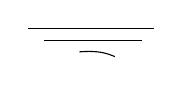
\begin{tikzpicture}[x=1cm,y=1cm]\draw (0,0)--(1.6,0);\draw (.2,-.16)--(1.45,-.16);\draw (.65,-.3)..controls(.9,-.28)and(1,-.32)..(1.1,-.36);\end{tikzpicture}}

\uline{Théorème} Soit $f:X-S$ morphisme de type fini, $S$ loc. noeth., $E$ cohérent sur $X$. Soit $F$ sur $S$ le \unsure{s-foncteur} de $\unsure{S|\underline{S}}$
\[
F(S')=\begin{cases}\varnothing&\text{si }F_{S'}\text{ non plat \inserted{(resp. non fid plat)} sur }S'\\\{\varnothing\}&\text{sinon}\end{cases}
\]
Pour que ce foncteur soit représentable, il \unsure{f.s.} qu'il commute aux limites projectives adiques d'anneaux artiniens.

Vérification des divers p\textsuperscript{ts}

1°) Faisceau pour fpqc Clair

2°) Commute aux $\varinjlim$ d'anneaux : EGA $\unsure{IV}$ 8 et $\unsure{IV}$ 11
\margin{$\times$ type fini \unsure{seul}, $F$ coh}

3°) Condition de commutation aux $\varprojlim$ d'artiniens

4°) 5°) 6°) Si $A\unsure{-|\to}A'$ injectif ($A'$ fini sur $A$ local artinien) alors $F(A)\longrightarrow F(A')$ bijectif i.e. $F(A')\ne\varnothing\Rightarrow F(A)\ne\varnothing$ i.e. $X_{A'}$ plat (fid plat) sur $A'\Rightarrow X_A$ plat (fid plat) sur $A$ EGA IV 11

7°) --- $F(T_0)\ne\varnothing$, $F(U)\ne\varnothing\Rightarrow F(T)\ne\varnothing$ i.e. $X_{T_0}$ plat et $X_U$ plat $\Rightarrow X_T$ plat EGA IV 11.
\mspage{10}
\scanpage{12}
8°) --- Trouver $U$ ; il suffit encore que $X_{U_0}$ soit ``ess. libre'' sur $U_0$, OK par EGA IV 11

La condition énoncée dans le th. signifie ceci :

$(L)$ Pour tt $T$ spectre d'un anneau de \deleted{valuation discrète} \inserted{local noeth.}, [complet à corps résiduel alg. clos si on y tient, \deleted{\unsure{tout}} \unsure{tels} que $F_T$ sur $X_T/T$ soit plat sur $T$ dans un voisinage de la fibre générique [resp. et $F_{T_0}\ne0$, où $T_0$ le pt fermé\ldots], \deleted{alors} $E_T$ est plat sur $T$, \deleted{\unsure{Exemple}}
\margin{\figure{\begin{tikzpicture}\draw (0,3)..controls(.45,3.2)and(.35,2.9)..(.35,2.2)..controls(.3,1.7)and(.35,1.65)..(.7,1.5)..controls(.32,1.25)and(.32,1.05)..(.3,.5)..controls(.3,.1)and(.2,.1)..(-.2,-.1);\end{tikzpicture}}\uline{N.B.} On peut supposer $\dim T=1$ \deleted{$T$ irréductible} $T$ \unsure{irréduc.|primaire} i.e. $\operatorname{Ass}\underline{O}_T$ réduit à un \unsure{élément|point}, et $T_{\mathrm{réd}}$ Spec d'un anneau de valuation discrète\ldots}

\uline{Corollaire 1} O.K. si $f:X-S$ est \uline{propre}.

\uline{Corollaire 2} O.K. si \deleted{$\unsure{G}$} $F=\underline{O}_X$, $X$ un préschéma \uline{en groupes} sur $S$, satisfaisant la condition $R$ plus haut ---

\uline{Corollaire 3} Soit $f:X\longrightarrow S$ un morphisme de \deleted{type fini, $S$ loc. noeth.} \inserted{prés. finie}. Conditions équivalentes

(i) $f$ se factorise en $f'f''$ : \inserted{\deleted{$X\longrightarrow\unsure{S'}\longrightarrow S$, $S'$ \unsure{loc. noeth.}}} avec $f''$ fid plat, $f'$ \uuline{imm}

(i bis) \figure{
\begin{tikzpicture}[x=1cm,y=1cm]\draw (0,0)..controls(1,-.08)and(2,.03)..(3.4,.06);\end{tikzpicture}} avec $f''$ plat, $f'$ \unsure{imm|mono},

(ii) $\unsure{\varphi_2|p_2}$ de $X\times_S X\xrightarrow{\mathrm{pr}_1}X$ est \uline{plat}
\figure{
\begin{tikzpicture}[x=1cm,y=1cm]\draw[line width=.7pt](0,0)--(0,2);\draw[line width=.7pt](.06,0)--(.06,2);\end{tikzpicture}}
\mspage{11}
\scanpage{13}
Sous ces conditions, la factorisation (i) est unique à isom près, et $S'$ est de \deleted{t.f.} \inserted{prés. finie} sur $S$.

$(i)\Rightarrow(i\ \mathrm{bis})\Rightarrow(ii)$ triv. De $=$ l'unicité de la factorisation \inserted{(i)}, car $X\longrightarrow S'$ \unsure{surj. quac.}, donc couvrant pour fpqc donc $S'=X/R$, où $R=X\times_S X$.

Reste à prouver $(ii)\Rightarrow$ \inserted{le faisceau} $X/R$ est représentable par un $S'$ de \inserted{loc.} type fini sur $S$. \deleted{[N.B. alors \unsure{cela} \unsure{quasi compact} sur $S$ car $X\longrightarrow S'$ est}

[N.B. Alors $X\longrightarrow S'$ est couvrant pour fpqc, comme \unsure{après le chgt|on voit du. chgt} de base $X-S'$ \unsure{il|et} donne $X\times_S X=R\longrightarrow X$ qui est fid plat par hypothèse ; il est fid plat \unsure{par. cqt} lui-$=$, ce qui implique \inserted{aussi} que $S'$ est \inserted{\unsure{par. cqt loc.}} de t.f. \deleted{\unsure{donc quasi}\ldots})].

Or \deleted{\unsure{comme} $X/R\longrightarrow S$} le foncteur représenté par $X/R\unsure{\hookrightarrow|\leftarrow}S$ est ici le suivant :
\[
F(\unsure{T})=\begin{cases}\varnothing&\text{si }X_T\text{ non fid plat sur }T\ \inserted{[\Leftrightarrow X_T\longrightarrow T\text{ couvrant fpqc}]}\\\{\varnothing\}&\text{sinon}\end{cases}
\]
D'ailleurs on est ramené au cas $S$ affine, \uuline{noethérien}.
\deleted{et} Alors on applique le th., qui nous dit qu'il suffit de vérifier \deleted{\unsure{que}} $(L)$. Or sous la condition de cette condition, $X_T\longrightarrow T$ est couvrant [car il contient un pt \inserted{$x$} de la fibre spéciale, et $\operatorname{Sp}\underline{O}_{X,x}-\operatorname{Sp}\underline{O}_{T,t_0}$ est fid plat] donc on \unsure{gagne} !
\mspage{12}
\scanpage{14}
\uline{Exemple}

\uline{Corollaire} Soit $G$ un préschéma en groupes de \deleted{type} \inserted{prés} finie sur $S$, \deleted{loc. noeth.} $P$ un \deleted{fibré principal} préschéma de prés. finie sur $S$ dans lequel $G$ opère, de façon que $P$ soit form. pr. hom. sous $G$. Sous ces conditions, il existe un mono de préschémas $S'\hookrightarrow S$, tel que $P\longrightarrow S$ se factorise par $P-S'$, et que \deleted{\unsure{P de} $P'$} $P$ devienne \deleted{formellement} principal hom sous $G_{S'}$ i.e. $P\longrightarrow S'$ est \deleted{plat} \uline{fid.} \uline{plat}. [De \deleted{Et} plus, $S'$ est uniquement déterminé à $S$-isom près, et est de prés. finie sur $S$].

\uline{Corollaire} Soit $u:G-H$ un hom de $S$-préschémas en groupes, \deleted{\unsure{de présentation}} $u$ de présentation finie. Supposons $\operatorname{Ker}u=N$ [qui est de prés. finie sur $S$] \uuline{plat} sur $S$. \uline{Alors} \deleted{\unsure{$u$ se factorise}} $G/N$ \uline{existe}.
\figure{
\begin{tikzpicture}[x=1cm,y=1cm]\draw (0,0)--(.02,2.6);\end{tikzpicture}}
\mspage{13}
\scanpage{16}
\diagram{\begin{tikzcd}Z\arrow[r,"\varphi"]\arrow[dr,"\deleted{\varphi}h"']&X\arrow[d,"f",no head]&Y\arrow[dl,"g",no head]\\&S&\end{tikzcd}}
\diagram{\begin{tikzcd}Z'\arrow[r,"\varphi'"]\arrow[rr,bend left=25,"v"]\arrow[dr,"h'"']&X'\arrow[r,"u"']\arrow[d,"f'"]&Y'\arrow[dl,"g'"]\\&S'&\end{tikzcd}}
\margin{Énoncer plutôt en termes de $\prod_{X/S}P/X\longrightarrow\prod_{Z/S}\unsure{Q}/Z$}
\figure{\begin{tikzpicture}[x=1cm,y=1cm]\draw (0,0)--(5.1,0);\draw (2.4,0)--(2.44,1.8);\draw(.95,-.18)--(.96,-.7);\end{tikzpicture}}

$f,h$ plat et propre sur $S$ loc. noeth

$g$ \deleted{\unsure{séparé}} de type fini [et séparé !]
\margin{\figure{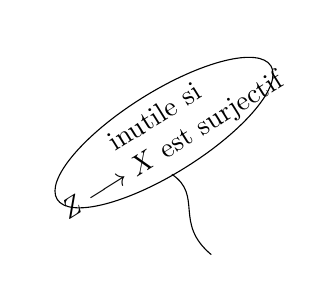
\begin{tikzpicture}\node[rotate=32,align=center] at(0,0){inutile si\\$Z\longrightarrow X$ est \uline{surjectif}};\draw[rotate=32](0,0)ellipse(1.6 and .52);\draw(.1,-.53)..controls(.5,-.8)and(.12,-1.15)..(.6,-1.55);\end{tikzpicture}}}
\margin{\uline{N.B.} l'hypothèse $S$ loc. noeth peut être remplacée par des hypothèses de présentation finie sur $f,g,h$.}
\unsure{a un mor}
\diagram{\begin{tikzcd}[cells={nodes={draw=gray,ellipse,inner xsep=8pt,inner ysep=5pt}},column sep=large]\underline{\operatorname{Hom}}_S(X,Y)\arrow[r]&\underline{\operatorname{Hom}}_S(Z,Y)\end{tikzcd}}
Pour $\varphi$\ldots

a) Le sous-foncteur de $\underline{\operatorname{Hom}}_S(X,Y)$ où $\underline{\operatorname{Hom}}_S(X,Y)$ est non \uline{ramifié} sur $\unsure{\varphi}$ \inserted{$\underline{\operatorname{Hom}}(Z,Y)$}, est un sous-foncteur ouvert.

Il correspond à $u':X'\longrightarrow Y'$ tel que, pour tout $s\in S'$,
\[
\operatorname{Hom}(u_s^{\unsure{\prime|\circ}*}(\Omega^1_{Y'_s/k(s)}),k(s))-\operatorname{Hom}(v_s^{\unsure{\prime|\circ}*}(\Omega^1_{Y'_s/k(s)}),k(s))
\]
est injectif. \uline{Or} on peut trouver sur $S'$ des Modules \uline{cohérents} $M_u,M_v$ tels que pour tt $J$ qu. coh. sur $S'$, on ait des isom \unsure{fonctoriels|naturels}
\[
\operatorname{Hom}_{\underline{O}_{X'}}(u^*(\Omega^1_{Y'/S'}),\unsure{\underline{O}_{X'}|f_{X'}}\otimes_{\underline{O}_{S'}}J)\simeq\operatorname{Hom}_{\underline{O}_{\unsure{S|S'}}}(M_u,J)
\]
\[
\operatorname{Hom}_{\underline{O}_{Z'}}(v^*\Omega^1_{Y'/S'},\underline{O}_{Z'}\otimes_{\underline{O}_{S'}}J)\simeq\operatorname{Hom}_{\underline{O}_{\unsure{S|S'}}}(M_v,J)
\]
\margin{N.B. \uline{\unsure{réduction}} \uline{immédiate} \uline{au cas} $S'$ \uline{artinien}}
et la formation de $M_u,M_v$ est compatible avec l'extension de la base. Ceci dit, on a un hom naturel
\[
(*)\qquad M_v\longrightarrow M_u
\]
qui définit par $\operatorname{Hom}(\ ,J)$ l'hom naturel
\[
\operatorname{Hom}_{\underline{O}_{X'}}(u^*\Omega^1_{Y'/S'},\underline{O}_{X'}\otimes_{\underline{O}_{S'}}J)\longrightarrow\operatorname{Hom}_{\underline{O}_{Z'}}(v^*\Omega^1_{Y'/S'},\underline{O}_{Z'}\otimes_{\underline{O}_{S'}}J).
\]
Dire \deleted{Alors} \inserted{que} la condition de non ramification est satisfaite en un pt $s\in S'$, signifie qu'en ce point
\[
M_v\otimes k(s)\longrightarrow M_u\otimes k(s)
\]
est \uline{surjectif}, et par Nakayama ceci restera vrai en
\mspage{15}
\scanpage{17}
voisinage.
\figure{
\begin{tikzpicture}[x=1cm,y=1cm]\draw[gray](0,.37)--(.7,.5);\draw[gray](.05,.3)--(.68,.4);\draw[gray](.25,0)--(.27,.43);\draw[gray](.61,.06)--(.64,.46);\end{tikzpicture}}

Nous désignerons par
\[
F=F_\varphi=\underline{\operatorname{Hom}}_S(X,Y;\varphi)
\]
le sous-foncteur précédent de $\underline{\operatorname{Hom}}_S(X,Y)$, dont la valeur en $S'$ est l'ens des \unsure{$S'$-homs} $u:X'-Y'$ tels que, posant $v=u\varphi'$, et considérant $M_v^{\unsure{\cdot|\prime}},M_u,M_v\longrightarrow M_u$ correspondant, $M_v\longrightarrow M_u$ soit surjectif.

\uline{Théorème} $\underline{\operatorname{Hom}}_S(X,Y;\varphi)\longrightarrow\underline{\operatorname{Hom}}_S(Z,Y)$ est représentable par morphismes non ramifiés.
\figure{\begin{tikzpicture}[x=1cm,y=1cm]\draw[gray](0,0)..controls(.4,.45)and(.7,.25)..(.95,.04);\draw[gray](2.3,.03)..controls(2.4,.45)and(3,.32)..(3.45,.08);\end{tikzpicture}}

\uline{Corollaire} Si $\underline{\operatorname{Hom}}_S(Z,Y)$ est représentable, alors $\underline{\operatorname{Hom}}_S(X,Y;\varphi)$ l'est également, et le morphisme $\underline{\operatorname{Hom}}_S(X,Y;\varphi)-\underline{\operatorname{Hom}}_S(Z,Y)$ est non ramifié
\figure{
\begin{tikzpicture}[x=1cm,y=1cm]\draw (0,0)--(-.04,1.2);\end{tikzpicture}}

\uline{Principe de la démonstration} On peut supposer donné un $v:\operatorname{Hom}_S(Z,Y)$, et on doit représenter le sous-foncteur de $\operatorname{Hom}_S(X,Y)$ dont la valeur en $S'$ est l'ens des $S'$-morphismes $u':X'-Y'$ tels que 1°) $u'\circ\varphi'=v'$ 2°) La condition $M_{v'}\longrightarrow M_{u'}$ surjectif. On applique le critère général de représentabilité \inserted{pour} des \deleted{foncteurs}
\margin{N.B. Réduction au cas $S$ noeth. immédiate \unsure{sans doute sur} foncteurs rel. représentables}
\mspage{16}
\scanpage{18}
préschémas \deleted{loc. de type fini} \inserted{non ramifiés} séparés sur $S$. \unsure{Seules|Toutes} les \inserted{deux dernières} conditions de modularité se vérifient par des techniques habituelles. \deleted{\unsure{On a des}} Celle au point \uline{générique ne doit pas faire} d'ennuis, avec le calcul habituel d'obstructions.
\margin{\uline{Tout} \uline{\unsure{reste}} à \uline{\unsure{rédiger}}}
\figure{\begin{tikzpicture}[x=1cm,y=1cm]\draw (0,0)--(2.6,.05)..controls(2.85,.06)and(2.85,.26)..(2.85,.45)--(5.2,.5);\draw (.35,-.25)..controls(.43,-.17)and(.47,-.37)..(.57,-.27);\end{tikzpicture}}

Reste le cas où $S$ est local noeth \inserted{irréductible} de dim 1, avec Idéal $J$ annulé par le nilradical, d'où $S_0=V(J)$, et où on dispose de $u_0:X_0\longrightarrow Y_0$ (tel que $u_0\varphi_0=v_0$) et un prolongement $u_\eta:X_\eta-Y_\eta$ ($\eta$ le pt générique de $S$) tel que $u_\eta\varphi_\eta=v_\eta$, $u_{\eta0}=u_{0\eta}$. Question de prolonger $u_0$ en $u$ tel que $u\varphi=v$. \deleted{\unsure{on}} Soient $P(u_0,S),P(u_0,S_\eta);P(v_0,S),P(v_0,S_\eta)$ les prolongements de $u_0$ resp. $v_0$ sur $S$, \deleted{et} de $u_{0\eta}$ resp. $v_{0\eta}$ sur $S_\eta$, d'où le diagramme comm
\figure{
\begin{tikzpicture}[x=1cm,y=1cm]\draw (0,0)--(-.03,1.3);\end{tikzpicture}}
\diagram{\begin{tikzcd}P(u_0,S)\arrow[r]\arrow[d]&P(u_0,S_\eta)\quad *\arrow[d]\\{}_*P(v_0,S)\arrow[r,no head]&P(v_0,S_\eta)\end{tikzcd}} $(1)$
\unsure{d'ens} \unsure{form.} princ. homogènes sous les groupes
\diagram{\begin{tikzcd}\operatorname{Hom}(M_{u_0}^{\unsure{*|\prime}},J)\arrow[r,no head]\arrow[d]&\operatorname{Hom}(M_{u_0},J_\eta)\arrow[d]\\\operatorname{Hom}(M_{v_0},J)\arrow[r]&\operatorname{Hom}(M_{v_0},J_\eta)\end{tikzcd}} $(2)$
Par hypothèse on \unsure{tient} des \unsure{élémts|éléments} aux coins
\mspage{17}

\end{document}
